\section{Experimental Setup}
\label{sec:exp-setup}

\cmtDK[inline]{15 pages}

In this section I will describe which experiments were conducted to answer the \cmtDK{?}{questions} from the previous sections as well as the setup of these experiments.
This will be done in two parts.
The first part contains the creation of the datasets that will be used in the experiments.
In the second part I will go deeper into discussing each experiment, including the necessity of the experiment, which datasets the model is trained on, as well as the final architecture of the models.

\subsection{Creation of the dataset}
The basis for my datasets is the CLEVR dataset \citep{Johnson2016}.
This dataset includes 3D-generated images depicting scenes with different kinds of objects.
Each of these objects has different combinations attributes, such as \emph{shape}, \emph{color}, \emph{size} and \emph{material}.
The possible values of these attributes are listed in Table \ref{tab:clevr-attributes}.
Three to ten objects are randomly placed into the scene and assigned with random attributes.
To enhance realism and reduce ambiguity, objects do not intersect, have a certain distance from each other, and are at least partially visible.
Figure \ref{fig:clevr-example} shows an example of a generated image in the CLEVR dataset.

\begin{table}[h]
    \centering
    \begin{tabular}{cccc}
        \toprule
        \textbf{ shape } & \textbf{ color } & \textbf{ size } & \textbf{ material } \\
        cube             & gray             & small           & rubber              \\
        sphere           & red              & large           & metal               \\
        cylinder         & blue                                                     \\
                         & green                                                    \\
                         & brown                                                    \\
                         & purple                                                   \\
                         & cyan                                                     \\
                         & yellow                                                   \\
        \bottomrule
    \end{tabular}
    \caption{Attributes of objects in the CLEVR dataset}
    \label{tab:clevr-attributes}
\end{table}

\begin{figure}[h]
    \centering
    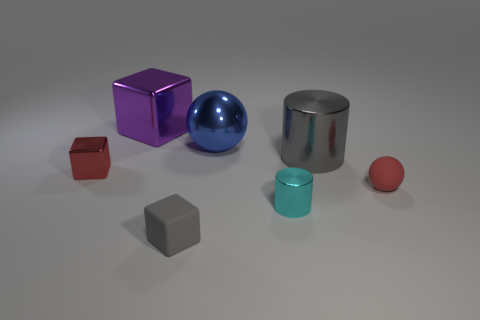
\includegraphics[width=.8\linewidth]{figures/CLEVR_example.png}
    \caption{Example of a generated image in the CLEVR dataset}
    \label{fig:clevr-example}
\end{figure}

Furthermore, the dataset contains information about each scene.
This includes all selected attributes for each object as well as the exact position of the centers of all the objects, both 3D-coordinates in the 3D scene and 2D-coordinates in the final rendered image.
In addition, simple spatial relations (in front of, behind, left, right) between the objects are calculated and stored.
These are simply based on the 3D-coordinates of the objects in relation to the position of the camera.

\cmtDK{ambiguity}
\cmtDK{referring expressions}

This research investigates how agents communicate about the relations of objects seen in images.
For that reason, the original CLEVR dataset offers too little control over how the objects are created and in which relation they stand to each other.
Following, I extended the source code to generate images for the CLEVR dataset.\footnote{\href{https://github.com/DominikKuenkele/MLT\_Master-Thesis\_clevr-dataset-gen}{https://github.com/DominikKuenkele/MLT\_Master-Thesis\_clevr-dataset-gen}}
To simplify the generation and the later learning of the models, I only focused on the attributes with a high impact on the appearance of the object, namely the \emph{shape}, \emph{size} and \emph{color}.
The \emph{material} is always the same for all objects in a generated image.
There were three main extensions to the code:

First, objects in the scene were separated into three categories: one \emph{target object}, objects in a \emph{target group} and \emph{distractor} objects.
The target object is the main object in the scene that should be identified and communicated by the agents.
All other objects and their relations are based on this target object.
The target group contains similar objects to the target object.
These are objects that the agents need to discriminate the target object from.
Finally, the distractors are objects that add noise to the scene and should make it more complex. They expected to teach the agents more precise descriptions of the target object.
The number of the objects in both group can be controlled.

In a second step, when generating the images it is possible to define the relations between \emph{target object}/\emph{target group} and \emph{target object}/\emph{distractors}.
The relation is defined as \textbf{how many} attributes of the target object are identical with the attributes of a single object in the target group and distractors respectively.
For example the target object is a \emph{small red cube}.
If two attributes are shared between target object and target group, objects in the target group could include \emph{small blue cube}, \emph{big red cube} or \emph{small red sphere}, but couldn't include another \emph{small red cube} or a \emph{small blue cylinder}.
The number of shared attributes can also be set to a range to make the discrimination task more challenging.

Lastly, it is also possible to define exactly \textbf{which} attributes should be shared between the target object and the groups.
For example, it can be defined to have the same size for objects in the target group, but have different, randomly selected shapes and colors.
This allows for a very controlled generation of relations between the objects in the scene.
Figure \ref{fig:clevr-dale-5} shows one generated image with this extended source code.
Here, the target object is the large purple cylinder.
The target group contains four objects that share zero to a maximum of two attributes.
It is not controlled, which attributes are shared (they are selected randomly). The large purple cylinder shares the same color and size with the large purple sphere, the same size with both cubes and no attribute with the small turquoise sphere.
There are no distractor objects.

For all generated datasets in the following sections, the general constraints and settings are as close as possible to the original CLEVR dataset.
The size of the generated images is 480x320 pixels.
10.000 images are created for each of the datasets.
Each image contains a maximum of 10 objects, that are not intersecting, have the same minimum distance between objects and are partially visible from the camera.

\begin{figure}[h]
    \centering
    \subfigure['CLEVR single', \emph{large yellow sphere}]{
        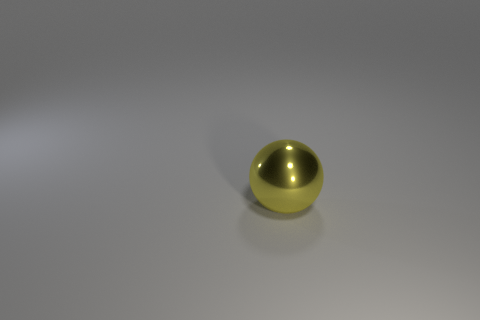
\includegraphics[width=0.43\linewidth]{figures/CLEVR_single.png}
        \label{fig:clevr-single}
    }
    \subfigure['CLEVR color', \emph{small brown cylinder}]{
        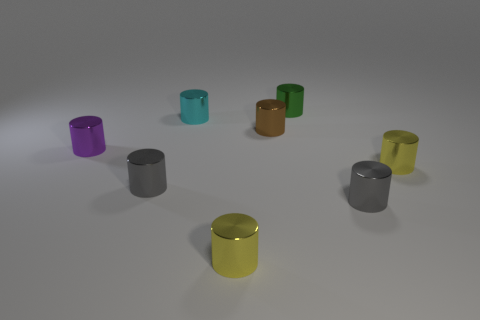
\includegraphics[width=0.43\linewidth]{figures/CLEVR_color.png}
        \label{fig:clevr-color}
    }
    \subfigure['Dale-2', \emph{small green cylinder}]{
        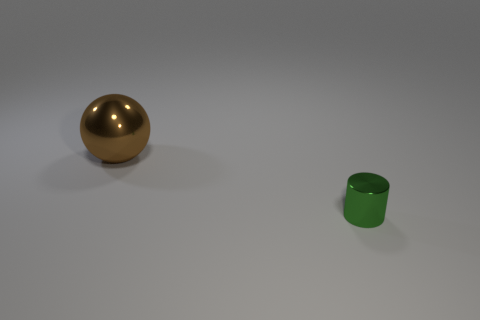
\includegraphics[width=0.43\linewidth]{figures/CLEVR_dale-2.png}
        \label{fig:clevr-dale-2}
    }
    \subfigure['Dale-5', \emph{large purple cylinder}]{
        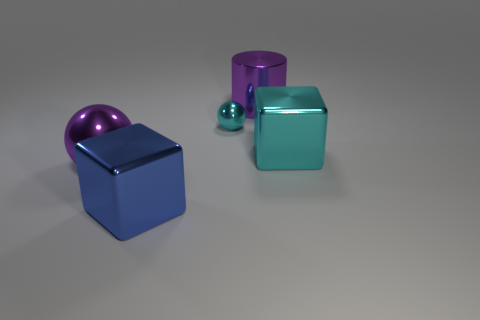
\includegraphics[width=0.43\linewidth]{figures/CLEVR_dale-5.png}
        \label{fig:clevr-dale-5}
    }
    \caption{Example images of each dataset, with the target object specified}
    \label{fig:clevr-examples}
\end{figure}

\subsubsection*{CLEVR single}
The simplest dataset is called 'CLEVR single'.
This is a very simple dataset and has the purpose to simplify the problem the model needs to learn as much as possible.
Each scene in the dataset contains only one single object, the target object.
There are neither objects in the target nor in the distractor group.
All attributes are assigned randomly to the target object.
The differences across the whole dataset are the locations and rotations of the objects.
With this dataset, neural models can focus on only the features, as well as the locations of this single object.
There are no objects that distract the model from extracting features from the target object.
This helps to understand if the models are actually able to assign features or learn locations of these features in an image.
Figure \ref{fig:clevr-single} shows an example with the only object being the \emph{large yellow sphere}.

\subsubsection*{CLEVR color}
This task could on the other hand be difficult to learn for neural models.
Although the target object is unique in the scene with resect to the distractors, the description isn't.
Considering all unordered combinations of the three attributes and a composite referring expression, there are $\binom{3}{3} + \binom{3}{2} + \binom{3}{1} = 7$ possible descriptions of the target object.
This can propose a difficulty, when the models try to converge towards one representation.
For this reason, I created the 'CLEVR color' dataset.
It has a similar setup as the previous dataset, containing between 6 and 9 distractors.
But instead of the target object sharing no attribute with the distractors, they share exactly two attributes.
Furthermore, to simplify the relation between target object and distractors over the whole dataset, it is also controlled which attributes are shared.
The distractors have always the same size and shape as the target object, but the color is always different.
The reason for choosing the color as the only discriminating attribute is that it is assumed that the color is easier to learn for neural models as opposed to for instance abstract shapes.

As seen in Figure \ref{fig:clevr-color}, the \emph{small brown cylinder} is unique.
The number of possible descriptions is lowered to three, since the color \emph{brown} needs to be part of it.
Notice as well that this restriction doesn't apply to the distractors, where multiple objects with the same color are allowed.

\subsubsection*{CLEVR Dale datasets}
Both of the above described datasets are very restrictive on the disambiguating relations between the target object and the rest of the objects.
Either no attribute or only one attribute is shared.
More realistically would be if objects can share a variable number of attributes.
In real situations, there is no restriction at all, how objects or things relate to each other.
Natural language emerged that can refer to distinct attributes of these objects to discriminate them from each other.
This emergence of referring attributes and their combination is studied deeper in this work.

For this, I created a dataset that allows almost any relation between a target object and the distractors.
The relations are only restricted by the incremental algorithm for the Generation of Referring Expressions (GRE) described in \citet{Dale1995}.
This algorithm ensures that every scene contains a unique object in respect to its and the distractors' attributes.
Using the algorithm, one can refer to an object using its attributes to discriminate it from all other objects as efficiently as possible.
In other words, the object is described unambiguously using the lowest number of words.
For the dataset that means that zero, one or two attributes can be shared between the target object and distractor objects.
This ensures the uniqueness of the target object.
On the other side, it is not controlled which attributes are shared.
These are assigned randomly.
There is again no control over the relations between distractors, which means that distractors can appear multiple times.

Two datasets, following these rules are created.
The Dale-2 dataset contains one target object and one distractor (see Figure \ref{fig:clevr-dale-2}), while the Dale-5 dataset contains one target object and exactly four distractors.
Consider Figure \ref{fig:clevr-dale-5}, with the target object being the \emph{large purple cylinder}. The large purple sphere shares the size and color, the two cubes only share the size, and the small turquoise sphere doesn't share any attribute.

These two datasets allow a more realistic look in how models can acquire knowledge about attributes of objects.
More specifically how models learn to discriminate objects from each other, since the model may only need to learn discriminative features of objects and not all features of the whole object.

\cmtDK{probabilities of shared attributes for both Dale-2 and Dale-5}

\subsection{Description of experiments}
Language games are very complex setups for machine learning models.
The models need to solve multiple tasks at the same time to solve the overall problem.
For instance, in a simple setup of a game two agents are involved.
The first agent, the sender, is shown a scene with objects and needs to communicate one target object to the other agent, the receiver.
The receiver is shown the same scene and needs to identify the target object with respect to the message of the sender.
In this case, the sender first needs to learn to encode the scene, all objects and their attributes, as well as the information about the target object into its own \cmtDK{?}{space}.
In a next step it needs to learn how to translate this encoding into a message that is sent to the receiver.
The receiver then needs to learn to decode this message, after which it needs to learn how to combine the decoded message with its own encoding of the scene and objects.
And finally it needs to learn how to identify the target object with this information.

For this reason, I decided to divide the main problem and let the models learn simpler subtasks and increase the complexity step by step.
\footnote{\href{https://github.com/DominikKuenkele/MLT\_Master-Thesis}{https://github.com/DominikKuenkele/MLT\_Master-Thesis}}
This will give me a very detailed overview, where the models struggle to learn and in which ways they can be improved.
Mainly, I separated the tasks into language games with two agents (final experiments) and classical machine learning tasks without any communication, namely only one 'agent' that solves the task alone (pre-experiments).
With this division, I can analyze the learning of the encodings of the scenes separately from the learning of producing and decoding messages.

\subsubsection{Feature extractors}
To extract features from the images, I make use of different deep neural network architectures that are developed for this task.
First, I use the \cmtDK{why ResNet/VGG?} VGG19 \citep{Simonyan2015} which is an architecture based on many convolutional layers.
After the convolutional layers, the data is passed first through an average pooling layer which outputs 512x7x7 dimensions.
Next follow three linear layers with \emph{ReLU} non-linearities in between.
After flattening the input, these classification layers output 4069, 4069 and 1000 dimensions respectively.

Secondly, I include the ResNet-101 \citep{He2016} that tries to overcome problems of very deep networks, using \cmtDK{needs to be explained deeper?}{residual blocks}.
There are four blocks that output 256x56x56, 512x28x28, 1024x14x14 and 2048x1x1 dimensions.
A following average pooling layer outputs 2048x1x1 dimensions as well.
The final linear layer reduces the flattened data to 1000 dimensions, corresponding to the ImageNet classes.

Both architectures are available pretrained on an image classification task on the ImageNet dataset.
Since the task in this research is very different from a classification, multiple different adaptions of these architectures are compared. \cmtDK{deeper discussion about different layers of these networks}
Table \ref{tab:feature-extractor-archs} lists the different adaptions for both VGG19 and ResNet-101 that will be used in this research.
In the later chapters, it will be referred to these adaptions using the name in the table.

\begin{table}[h]
    \centering
    \begin{tabular}{rlc}
        \toprule
                            & \textbf{description}                                            & \textbf{ output dimensions } \\\midrule
        \textbf{VGG-0}      & contains only the convolutional layers                          & 512x7x7                      \\
        \textbf{VGG-avg}    & contains an additional average pooling layer                    & 512x7x7                      \\
        \textbf{VGG-cls1}   & \makecell[cl]{contains an additional one classification layer,                                 \\ including its non-linearity} & 4069                         \\
        \textbf{VGG-cls2}   & \makecell[cl]{contains another additional classification layer,                                \\ including its non-linearity} & 4069                         \\
        \textbf{VGG-cls3}   & the original VGG19 architecture                                 & 1000                         \\\midrule
        \textbf{ResNet-1}   & contains one residual block                                     & 256x56x56                    \\
        \textbf{ResNet-2}   & contains two residual blocks                                    & 512x28x28                    \\
        \textbf{ResNet-3}   & contains three residual blocks                                  & 1024x14x14                   \\
        \textbf{ResNet-4}   & contains four residual blocks                                   & 2048x1x1                     \\
        \textbf{ResNet-avg} & contains an additional average pooling layer                    & 2048x1x1                     \\
        \textbf{ResNet-cls} & the original ResNet-101 architecture                            & 1000                         \\
        \bottomrule
    \end{tabular}
    \caption{Different adaptions of VGG19 and ResNet-101 used in this research}
    \label{tab:feature-extractor-archs}
\end{table}

Furthermore, I experimented with both the pretrained models as well as with the architectures trained from scratch with a random initialization for the weights.
This reason for this was to test if the success of an experiment was actually making use of the pretrained knowledge incorporated in the models.
If that was not the case, the agents were likely not using image features, but instead relying on some other underlying patterns to solve the task.
Basically, this approach works as an indicator to determine the actual success of the agents aside from measures as the accuracy or precision.


\subsubsection{Pre-experiments without language games}
The final objective of this thesis is to find out, how agents can communicate about relations of objects spatially as well as based on their attributes.
Because of that, the first experiments focus on extracting information from images and combining them with structured knowledge.
Here, I structured the experiments into three levels.
In the first level, the model are trained to learn the position of objects in the image and attend to specific regions of the image.
In the second level, the models are trained to differentiate objects in the scene from each other.
The last level adds language to the experiment, more specifically the models learn to caption and describe objects in the image.
These combined experiments should lay the basis for how to build up the agents in the language games.

\paragraph{Level 1 - Coordinate predictor:}

This level should help to analyze, how the final task of the language game should look like, in especially what the receiver is tasked to predict.
As described before, the sender should communicate an object in the image and the receiver needs to identify it.
The challenge lies in how the receiver refers to the identified object.
There are multiple possibilities, how it can be done.
One of them could be to describe the target object with human language, using the attributes.
The main goal however is to let the language of the agents emerge as natural as possible.
Including human knowledge into the task would bias also the emerged language towards attributes and words, humans are using.
For this reason, the final task of the receiver will be to 'point' to the target object.
Since also positional information of the objects should be part of the discrimination, the image will not be separated into several bounding boxes around the objects, but instead the whole image is the basis.
The models are therefore tasked to predict the center coordinates of the target object.
With this approach, the models receive few human knowledge, but are still able to rely on all information present in the image to discriminate the objects.

To achieve this goal, multiple setups of models are tested.
In the simplest setup, the model receives only the image \cmtDK{preprocess image} as an input and produces two numbers as an output, the predicted x- and y-coordinate of the target object.
Here the image is first passed through one of the \emph{feature extractors}.
Next, the extracted feature vector is flattened and passed through two linear layers with a \emph{ReLU} non-linearity between.
These reduce the dimensions first to 1024 and finally to 2.

To determine the loss, the euclidean distance between the resulting predicted point on the image and the ground truth point are calculated.
This distance is learned to be minimized.
By doing that, the model learns to focus and attend on a specific part in the image, in a perfect model the center of the target object.

With this simple setup, the model is in theory able to focus on an object in the image.
The problem arises as soon as multiple objects are present in the image.
There is no information available for the model to understand which one of these objects is the actual target object, except for the final calculation of the loss.
Since there is not necessarily a pattern for which object in the image is the correct target object over the whole dataset, the models will likely fail to generalize. \cmtDK{go deeper, why}
Therefore, the models need to receive more information.
Here, I try out four different ways to encode the target object.

In the first method, I encode the attributes of the target object as \textbf{one-hot encodings}.
There is a three-dimensional vector encoding the \emph{shape}, an eight-dimensional vector encoding the color and a two-dimensional vector encoding the two different sizes.
The dimensions of these vectors can either be zero or one, depending on the attributes of the target object.
These three encodings of the attributes are then concatenated.
The image is again passed through a feature extractor, before the flattened vector is reduced to 2048 dimensions with a linear layer.
The result is concatenated with the encoded attributes and passed to a final linear layer to predict the coordinates.

In an extension to this method, I also include the \textbf{center coordinates of all objects} in the image.
This should help the model to identify all possible options to chose from, when predicting the target object.
All the center coordinates are simply extracted and shuffled.
Since there are varying numbers of objects in the image, this vector of variable length is padded to 10 objects, resulting in a vector with a length of 20.
The padding objects have zeros for both coordinates, which no other real object can have.
For this model, I also made use of a more complex way to encode the image.
Here, I based the approach on code that implements baselines for the CLEVR dataset \citep{Johnson2017}. \cmtDK{why?}
The image is first passed through the feature extractor.
Afterwards, a 2-dimensional convolutional layer, reduces the channels from 2048 to 512 channels with a kernel size of 1.
After applying the \emph{ReLU} function, the resulting matrix is max pooled over two dimensions with both a kernel size and a stride of 2.
The resulting matrix is flattened and concatenated with both the attribute encodings and the shuffled coordinates of all objects.
This is then passed again through a final linear layer to predict x- and y-coordinates.

The third method encodes the attributes of the target object with human language using the \textbf{incremental algorithm for the Generation of Referring Expressions (GRE)} described in \citet{Dale1995}.
This opposes the idea described before, to share as few human knowledge as possible with the model.
Still, this approach can help to understand and analyze if the model was able to extract information about the objects and more specifically their attributes from the image.
If the model is able to match parts of the image with human words it would show that the model learned this attribute.
If the model in a next step can learn this over the whole dataset, this would mean that it could generalize over these attributes and assign them to certain regions in an image.
This insight could help then to design another model that makes use of these learnings without human language.

Using the algorithm, one can describe an object using its attributes to discriminate it from other objects as efficiently as possible.
In other words, the object is described unambiguously using the lowest number of words.
The algorithm assumes that there is an order of importance for attributes, such as shape, color and size.
This order defines, which attributes can be left, while still identifying the object uniquely.
For our research, we rely on the following order from most important to least important: shape, color, size
Given for example the scene from \ref{fig:clevr-dale-5} with the target object being the \emph{big purple cylinder}.
Using all three attributes, this description identifies the object perfectly and uniquely.
Following the algorithm, we could make the description shorter by removing the least important attribute \emph{size} without loosing unambiguity, describing it as the \emph{purple cylinder}.
This can be taken even one step further by removing also the \emph{color}.
Describing it as the \emph{cylinder} still doesn't describe any other object, since the target object is the only cylinder in the scene.

For the experiments, each every image is captioned, by a description of the target object using the described algorithm.
To use it in the model, the caption needs to be padded to an equal length, in this case to a length of 3, which is the maximum number of attributes that can be used.
For this, as standard practice in captioning tasks, the captions are padded at the end with a specified padding token.

The model is made up of three parts:
The first part extracts features from the image.
Here, the setup is similar to the previous model.
The image is passed through a feature extractor, before it is passed through two 2d convolutional layers, both reducing the channels to 128 with a kernel size of 1.
A \emph{ReLU} function is applied, after both convolutional layers.
As before, the resulting vector is pooled, using max pooling with both a kernel size and stride of 2.
In the second part, the caption is encoded, using an LSTM.
Here, the learned embeddings of each token are parsed by the LSTM and its final hidden state is then used as a summary of the complete caption.
The third part is again the predictor of the coordinates of the target object.
Both the processed image and the final hidden state of the LSTM are flattened and concatenated.
The resulting vector is passed through three linear layers reducing to 1024, 1024 and 2 dimensions respectively.
Between each linear layer, the \emph{ReLU} function is applied.
This architecture is also inspired by the baselines described in \citet{Johnson2017}.

The forth method, to encode the target object utilizes \textbf{masking} of the image.
For this, the image is separated into a fixed size squared area containing the target object and the rest of the image.
The side of the square is always two fifth of the image width, in this case 192 pixels.
This size always includes the whole object if it is large or small, while not being cut of if the target object is too close to the border of the image.
The square is filled in white, while the rest of the image is filled in black.
This approach has the advantage of providing as few as possible human bias to the model.
While even the one-hot encodings contain human knowledge by explicitly encoding human chosen attributes, masking the image will only point the model towards the target object without giving more information.
It therefore can only rely on its own extracted visual features when looking at masked images.\cmtDK{can just rely on masked image when predicting coords, more useful for captioning or language game}

The model is presented with both the original image and the masked image.
Both are passed through a feature extractor and afterwards passed through a linear layer, reducing the dimensions to 2048.
The resulting vectors are concatenated and passed through another linear layer that predicts the coordinates.

The test dataset is again evaluated on the euclidean distance of the predicted coordinates to the ground truth coordinates.
This distance needs to be minimized.
The mean of all calculated distances is calculated across the whole epoch, which results in a mean distance score per epoch.
Since this score only takes the average of all predictions into account it can't evaluate every prediction individually.
If for instance the prediction of one object is getting more precise with growing number of epochs, but the precision of another object gets worse, the mean distance will stay the same.
It doesn't reflect this change.
For that reason, I also introduced an accuracy score.
For that I defined a fixed size circle with a radius of 20 pixels around the center of each object.
If the model's prediction lies in this circle, it will be counted as a correct prediction, if it lies outside, it is a false prediction.
These scores are averaged for the epoch and result in an accuracy score, where 100\% means that all predictions were very close to the center coordinates and 0\% means that no predictions were close to the center coordinates.
This of course doesn't give a perfect representation since the size of the objects varies, but it will still show, how precise each individual prediction is.
A high accuracy may indicate that the model could identify this specific object better.

The coordinate predictors are trained on the 'CLEVR single' as well as on both 'Dale' datasets.
The 'CLEVR single' dataset should test the model if it can actually learn locations of an object.
Since the model relies on the extracted features of either VGG or ResNet, locational information about the image could have gone lost.
Training on this dataset should make sure that the model can converge towards the correct pixels, utilizing these features.
In a next step, the 'Dale' datasets provide the actual problem of discriminating objects from each other and afterwards pointing to the correct one.
Here, the models should make use of the additional given information about the scene, as one-hot encodings of the attributes, descriptions using the GRE-algorithm or the encoded locations.
'Dale-2' and 'Dale-5' provide two different difficulties for the model, where it needs to discriminate a target object from one or four distractors.
Latter task is assumed to be significantly harder.

\paragraph{Level 2 - Bounding box classifier:}
\cmtDK{better to call it discriminators?}

One problem that arises, when only predicting the coordinates is that the models may not be able to predict locations of objects from just visual features.
Feature extractors like VGG or ResNet are trained on extracting visual information.
In this process, absolute locations of these features in the images may get lost in the resulting vectors, since they are not important for this task.
To address this challenge, I restructured the task in this experiment.
Instead of predicting two coordinates of a target object, the model now needs to classify between all available objects.
This will take all positional information out and just focus on the attributes and discriminating factors between the objects.
To do this, fixed-size bounding boxes are extracted around each of the object in the image.
As for the masking, the bounding boxes are a square of 192x192 pixels, to capture the complete object. \cmtDK{preprocess bounding box}
The bounding boxes of all objects are padded to a number of 10 bounding boxes, the maximum number of objects in an image with a matrix of zeros.
These bounding boxes are shuffled.

The model passes each of the bounding boxes through a feature extractor.
The resulting vectors are concatenated, which basically is a concatenation of the extracted features of each object.
This long vector is passed through a linear layer with 4096 with a subsequent \emph{ReLU} function.
Afterwards, a linear layer reduces the dimensions to 10, corresponding to the 10 bounding boxes in the input.
With a final \emph{softmax} function, the model then points to one of the bounding boxes as the target bounding box.
The loss is calculated using cross entropy.

The bounding box classifier is trained on all datasets excluding the 'CLEVR single'.
The 'Dale' datasets are directly comparable to each other for the similar setup of their creation.
Especially interesting is the effect of the increasing the number of distractors and the growing number of attributes that are needed to discriminate the objects.

\paragraph{Level 3 - Caption generator:}

As the bounding box classifier, the caption generator only acts as a learning step towards understanding, how the model can learn the attributes of objects.
It is used the same way to create the captions for each image as in the section above with the GRE-algorithm.
This method focuses even more on human knowledge and structure of language than the experiment above, since it is even the final task of the model.
There are some minor additions concerning the padding of the caption.
As before, the caption is padded to a number of three tokens, corresponding to the maximum of three attributes.

However, there are three different ways how the padding is applied.
First, the captions are, as usual in captioning tasks padded at the end with a specified padding token.
A problem could arise when the caption is not viewed as a natural language sentence, but as slots filled with tokens.
More specifically, following the GRE-algorithm, the last token in the caption is always the shape.
The second last token if existing describes the color, while the third last token if existing describes the size.
As soon as this sequence is padded at the end, these slots suddenly disappear.
A caption that only describes the shape, such as \emph{cube} will be padded to \emph{cube <pad> <pad>}, where the third last slot is filled up with the shape instead of the size.
Since in this task we are not focussing on producing natural language with a correct grammar, but focus instead of extracting attributes, having a slot structure could help the model to express the extracted attributes correctly.
For this reason, the second method of padding the caption is prepending the caption with padding tokens.
By this, the positions of the slots are preserved and if not specified just filled with a padding token.
The last variation concerns the order of producing each token.
When the captions are prepended, the model would need first produce two padding tokens, before it finally can produce a much more meaningful token for the shape.
This could be difficult to learn for a model, as the longer a sequence of tokens is, the more information about the beginning of the sequence gets lost.
Even though a sequence of just three tokens may not be long enough for this factor to be a problem, I experimented to reverse the caption.
Instead of producing for instance \emph{<pad> green sphere} as correct in English, the model would now need to produce \emph{sphere green <pad>}.
Notice that the padding token is again at the end of the generation, but the order of slots as well as the amount of information in the caption are still preserved.

Nonetheless, this helps to understand more detailed if and how the model discriminates objects.
Does it rely on the same attributes, humans are using, or does it find other important differences, or is it able to solve the task at all?

I compare two different models against each other.
The first model just takes the image as the input.
During training, also the ground truth caption is passed to the model.
The image is processed as in the section before.
First, it is passed through a feature extractor with two following 2d convolutional layers, reducing the channels to 128.
After each convolutional layer the \emph{ReLU} function is applied.
The result is pooled using max pooling and then reduced to 1024 dimension using a linear layer.
The such encoded image serves as the initial hidden state of an LSTM, which generates the caption.
During training the input sequence for the LSTM at each time step are embeddings of the tokens in the ground truth caption.
No teacher forcing is applied.
The output of the LSTM is passed through a linear layer at each step to determine logits over the symbols of the vocabulary.
The loss is calculated using cross entropy.
When testing, the LSTM always generates three tokens, with a start-of-sequence token as first input to the LSTM.
Each token in the sequence is determined, by selecting the highest logit in the output of each step in the LSTM.

Since with this approach, the model doesn't have any information about the target object, I extend it with a masked image.
As in the section above, a masked version of the image is created and passed to the model.
The model works exactly the same, except for the additional separate image encoder that encodes the masked image in the same way as the original image.
Both encodings are concatenated and then used as the initial hidden state for the LSTM.
This should point the model to which object to describe and discriminate from the other objects.

To test the success of the model, three measures are calculated.
The first measure is the \textbf{accuracy} if the model predicted every word in the caption correctly.
This gives a hint, how the model fares in general and also able to predict actually any of the attributes at all.
However, a 'false' prediction doesn't give much insight into why the model predicted a wrong caption.

It could be the case that the model predicted the correct shape, but wrong color.
Even worse, the model could have predicted more attributes than necessarily to uniquely identify the target object and didn't follow the rules of the GRE-algorithm.
For instance, consider the scene in Figure \ref{fig:clevr-dale-5}.
The correct caption is \emph{cylinder}.
If the model would predict \emph{purple cylinder}, the accuracy determines it as false as captioning \emph{large purple cylinder} as well \emph{small green cube}.
The first two descriptions identify the target object perfectly, but the model only didn't learn yet to leave unnecessary attributes out.
To mitigate this, I also include a \textbf{word-by-word accuracy}.
This measure calculates the accuracy not on sentence level, but on word level.
The first predicted caption of the model would yield a word-by-word accuracy of 66\% (including padding tokens), the second 33\%, while the third prediction would
yield 0\%.
This can give a better understanding of the errors the model makes.

With the \textbf{non-target accuracy}, I identify if the model described another object, which is not the target image.
This is basically an inverted accuracy score; the lower the score, the better the model fares.
For this I generated captions for all the non-target objects and distractors in the images using the GRE-algorithm.
If the generated description of the model describes an object that is not the target object, it gets assigned 100\%.
If not, independently of describing the target object, no object, or one of the objects insufficiently, it gets assigned 0\%.
Using this measure, I can get a quick overview if the model's problem lies in extracting and relating attributes or in understanding which of the presented objects is the target object.

The caption generator models are trained on both 'Dale' datasets.
Again, each of these datasets increases the complexity of the description.
While the referring expression for the 'Dale-2' datasets are generally shorter, expressions of the 'Dale-5' datasets need to be more specific and use more attributes.
Furthermore, the model needs to attend to many more locations in the image at the same time to find discriminating factors between those.

\cmtDK{align 'description', 'caption' and 'referring expression' over the whole section}

\subsubsection{Language games}
The experiments that are executed using language games have a similar structure as the pre-experiments, since those lied the basis for the language games.

The language games in this research have an asymmetric setup.
One agent, the sender is shown some information and needs to generate a message.
This message is received by the second agent, the receiver.
The receiver needs to parse this message and combine it with the information they are given as well.
The receiver then makes a prediction, which is compared to the ground truth.
The game is set up prosocial, which means that both agents receive the same loss based on the receiver's prediction.
All weights of the agents are adapted in the same way.
\cmtDK{Gumbel-Softmax vs REINFORCE}
\cmtDK{better in theoretical background?}
\cmtDK{vocabulary?}
\cmtDK{batch iterator}
All language games are set up and run in the EGG framework \citep{Kharitonov2019}, developed in PyTorch.
This framework consists of heavy configurable core that controls the generating and parsing of the message, the calculation of the loss and the rules, for how the weights of all neural models are trained.
The configuration includes for example a choice between single symbol and sequence messages with varying RNNs, a choice between Gumbel-Softmax relaxation and REINFORCE algorithms to learn neural models containing discrete symbols or an easy switch between different loss functions.
Furthermore, runs of games can be saved to analyze the used messages of the agents and how they change over the duration of the learning.

The framework is hereby setup in three levels.
Part of the lowest level are the \emph{agents} themselves.
The agents are neural models that need to be developed from scratch and define how, the agents process their input and combine it with the message (in case of the receiver) and what they output.
The second level are \emph{wrappers} that take care of generating and parsing the message.
The sender wrapper uses the output of the sender agent, to produce a message.
The receiver on the other hand parses the message received by the sender and passes the result as an additional input to the receiver agent.
The third level, the \emph{game} links all described parts together.
It provides the agents with the input and passes the message from the sender to the receiver.
Furthermore, it uses the output of the receiver and calculates the loss, which is then the basis for the adaption of the weights for both wrappers and agents.

For the following language games, the sender will always produce a sequence of symbols as a message, which the receiver will parse.
Gumbel-Softmax relaxation is applied to produce discrete symbols.
This is done using two LSTMs, an encoder LSTM in the sender wrapper and a decoder LSTM in the receiver wrapper.
The output of the sender agent is used as the initial hidden state for the encoder LSTM.
This LSTM is then producing symbols until it generates an end-of-sequence symbol.
This sequence is then passed to the receiver wrapper with its decoder LSTM.
Its hidden state is initialized randomly.
The received message sequence is processed symbol by symbol.
After each time, a symbol is processed by the LSTM, the resulting new hidden state is passed to the receiver agent as the parsed message.
The receiver agent is combining it with its representation of the image input and predicting an output.
The \emph{game} is afterwards calculating a loss for each of these outputs separately.
These losses are summed up to a total loss that is used to adapt the weights in both agents as well as in both LSTMs.

\cmtDK{always ResNet-3}

First, I will discuss \emph{discrimination games}, because they have the simplest setup.
Furthermore, other language games that research this topic use a very similar setup.
In the next step, I will look into caption generators that are set up as a language game.
Here, the sender describes the scene, while the receiver needs to generate a caption.
In the last step, I try to lose as much human bias as possible and the models are trained on just 'pointing' towards the target object, by again predicting its center coordinates.

\cmtDK{look at emerged language: distribution of vocab/ngrams, how do they relate to the images (clustering?)}

\paragraph{Discrimination games:}
In a discrimination game, the agents are presented with two or more images, one of these being the target image.
The sender needs to communicate this target image to the receiver by discriminating it from the other distractor images.
The receiver then needs to decide based on the message, which of the images is the target image.

The discrimination games in this research have a very similar setup as described in \citet{Lazaridou2016}.
The agents in this research resemble their \emph{agnostic sender} as well as their \emph{receiver}.
One central difference is the production of the message.
The main goal of their language game was the identification of the concept that and image was related to.
Therefore, the sender communicated only single-symbol messages to the receiver, which should describe the concept of the target image.
Opposed to that in this research, the agents are tasked to discriminate objects from each other based on their attributes.
It is therefore assumed that the sender will communicate these discriminative attributes.
For that reason, the sender is allowed to generate sequences as a message.

Both 'Dale' datasets are used to train the agents in this mode.
Similarly to the bounding box classifier, bounding boxes around each of the objects are extracted and fed to the game.
As in \citet{Lazaridou2016}, the sender receives the bounding box of the target object as the first image, while the rest of the bounding boxes are shuffled.
The sender is assumed to learn which of the input images is the target images by this approach.
The receiver receives the images in completely shuffled order.

\begin{figure}[h]
    \centering
    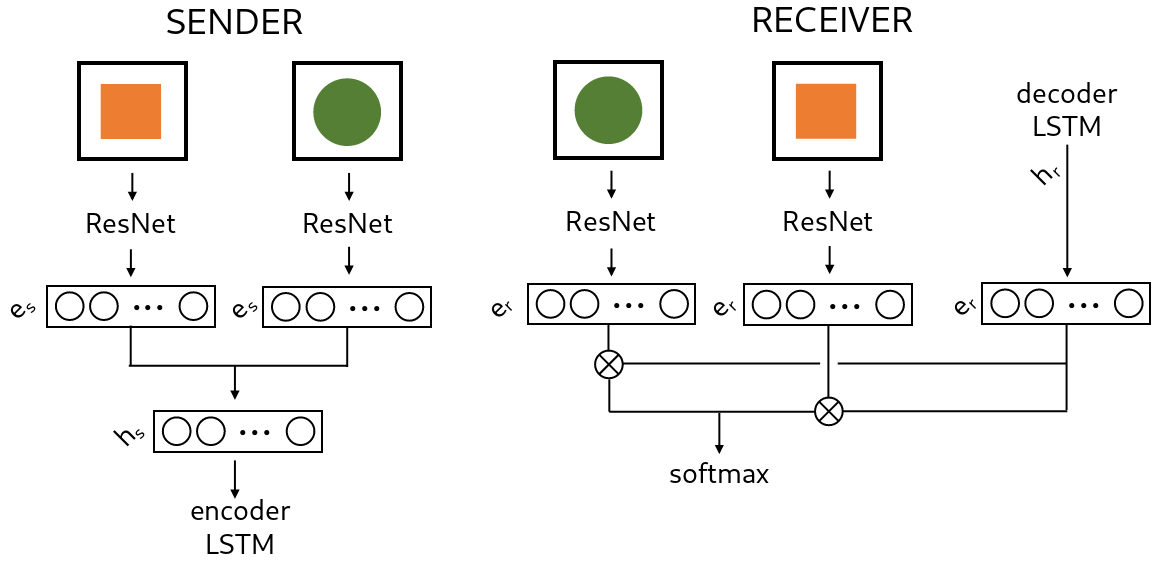
\includegraphics[width=.8\linewidth]{figures/discriminator.png}
    \caption{Sender and receiver architectures in the discrimination game}
    \label{fig:discriminator_architecture}
\end{figure}

Figure \ref{fig:discriminator_architecture} shows, how the sender and the receiver of the discriminator are built up.
For the sender, the images are passed through a feature extractor and a following linear layer that reduces the dimensions to an embedding size $e_s$.
All embedded images are concatenated and passed through another linear layer to reduce the dimensions to the hidden size $h_s$.
This is then used as the initial state of the encoder LSTM in the sender wrapper.

The receiver also encodes all images using a feature extractor with a following linear layer, reducing it to $e_r$.
The sequence, received by the sender is the input for its decoder LSTM, where the hidden state with a dimension of $h_r$ is randomly initialized.
As mentioned above, the receiver combines this image representation with the hidden state of each symbol separately.
This is done by passing the hidden state through a linear layer to scale its dimensions to the same $e_r$.
This allows the calculation of the dot product between it and the image representation.
If the message describes an object well, the resulting dot product should be higher.
The receiver then `points' to one of the images by applying the \emph{softmax} function over the results of the dot products.
The loss is calculated using the NLL-loss.

During the experiments, five variables are adjusted to compare their effects:
(1) the image embedding size for the sender $e_s$, (2) the LSTM hidden size for the sender wrapper $h_s$, (3) the image/message embedding size for the receiver $e_r$, (4) the LSTM hidden size for the receiver wrapper $h_r$ and (5) the size of the vocabulary $|V|$.

\paragraph{Caption generators:}
In a next step, it is tested if the agents can learn to extract features of the objects together.
For this, the receiver is tasked to describe the target object in natural language, while the sender needs to communicate, which object is the target.
Again, the setup is asymmetrical: the sender receives the image and information, which of the objects in the image is the target object in form of a masked image.
The receiver only sees the image without additional information.
\cmtDK{human bias vs emergent language}

This setup is based on the single neural model described above.
The target caption for each image is created using the GRE-algorithm of \citet{Dale1995}.
Since the results of the experiments show that the position of the padding doesn't have an effect on the final converging scores, the padding tokens are only prepended to the caption.

The sender is built up of two image encoders, one encodes the original target image and one encodes the masked image.
The image encoders are set up as described in \citet{Johnson2017}.
A feature extractor extracts basic features of the images.
Two following convolutional layers with a \emph{ReLU} function are trained to condense the most important information from the resulting matrices.
A max pooling layer and a linear layer reduce the dimensions to 1024 dimensions.
This size was found to have the best results during the experiments.
The two resulting encoded images are flattened and concatenated.
A final linear layer reduces this long vector to the hidden size of the message LSTM $h_s$, which is used as the initial hidden state of this LSTM.

The receiver uses the same architecture to encode the original image as the sender.
The resulting flattened vector is concatenated with the decoded message of hidden size $h_r$.
This is then passed through a linear layer, again reducing it to 1024 dimensions and is then used as the initial state of the captioning LSTM.
During training, the ground truth caption is used as the input to the LSTM without teacher forcing.
When presented with test data, the LSTM always produces three tokens, by using its own predicted words as the input for the next step.
The loss is calculated with cross entropy.

Since the agents are trained to describe the target object discriminatively based on the described GRE-algorithm, they are trained on the 'Dale-2' and 'Dale-5' dataset.
The 'Dale-5' should be again much harder to learn, since there are more objects that the agents need to discriminate the target object from.

During the experiments, the following variables are adjusted, and the results are compared:
(1) the vocabulary size $|V|$,
(2) the LSTM hidden size of the sender wrapper $h_s$ and
(3) the LSTM hidden size of the receiver wrapper $h_r$.
The same metrics as in the pre-experiments are used to evaluate the results.

\paragraph{Coordinate predictors:}
In the final experiments, it is tried to eliminate as much human knowledge as possible.
For that reason, the agents are tasked to only predict the location of the target object.
This task is approached in two steps.
In the first step the sender is still shown human knowledge in form of a description of the target object, since the previous experiments showed that the models were able to relate them to their own extracted features.
The receiver doesn't come in contact with any human knowledge, not as input nor as output.
This approach acts as a sanity check if the agents are able to converge together on the correct target object coordinates.
In the second step, the caption is also removed from the sender.
Instead, a masked image points the sender towards the target object.
In this setup, no human knowledge is explicitly present, that can bias the emerged language to form similarly to human language, except for the implicit information in the image itself.
With this, it can be analyzed, how the language between the agents emerges and which features or patterns are represented with symbols.

The agents are both set up in the same way as the single neural model, predicting the target object's coordinates.
The sender encodes the original image the same as in the previous paragraph.
In the first setup, the description of the target object is encoded, using an LSTM.
For this, an embedding with $emb_{descr}$ dimensions is learned to represent each word.
These embeddings are the input for the LSTM.
The final hidden state of $LSTM_{descr}$ dimensions is used as the representation of the whole description.
The vocabulary that is used for the descriptions is based on 14 symbols, including the padding token.
For the LSTM to learn a representation of each token as well as of the complete description, both $emb_{descr}$ and $LSTM_{descr}$ need to be smaller than the size of this vocabulary.
Choosing a size of 10 for both variables proved to give good results in the experiments.
In a next step, the image encoding and the final hidden state of the description are concatenated and passed through a linear layer to reduce the dimension to the hidden size $h_s$.
The resulting vector is passed to the sender wrapper LSTM, to generate the message.

For the second approach, the masked image is passed only through a feature extractor.
Both the resulting encoding of the masked image and the encoding of the original image are each passed through separate linear layer to adjust their dimensions to the same embedding size $e_s$.
These embeddings are subsequently concatenated and reduced to the hidden size $h_s$ with a final linear layer.

The receiver contains of two parts.
First, the original image is encoded with an image encode of the same setup.
This encoded image is flattened and concatenated with the final hidden state of the wrapper LSTM encoding the message received by the receiver.
The resulting vector is the passed through the second part of the receiver, the predictor.
This predictor contains of three linear layers, reducing the dimensions to 1024, 1024 and 2 respectively.
A \emph{ReLU} function is applied in between.
This setup is trained to combine the important information from both the image and the message of the sender.
The euclidean distance between the resulting prediction of the center point and the true center of the target object is calculated and the weights of both agents are adapted accordingly.

As in the pre-experiments, the agents are trained first the 'CLEVR single' dataset to understand if they are capable of predicting locations in an image together.
In a next step, the 'Dale-2' and 'Dale-5' datasets are used to test if the agents are able to first communicate a target object and second describe the target object discriminatively with a small vocabulary.

During the experiments, the effects of the following variables are compared:
(1) the vocabulary size $|V|$,
(2) the LSTM hidden size of the sender wrapper $h_s$,
(3) the LSTM hidden size of the receiver wrapper $h_r$ and
(4) the embedding size of the sender $e_s$.
As before, the metrics to evaluate the results are the same as in the pre-experiments.